\documentclass{article}
\usepackage[utf8]{inputenc}
\usepackage{graphicx}
\usepackage{amsmath}	% Advanced maths commands
\usepackage{amssymb}	% Extra maths symbols
\usepackage{amsfonts}

\usepackage{listings}
\usepackage{color}
 
\definecolor{codegreen}{rgb}{0,0.6,0}
\definecolor{codegray}{rgb}{0.5,0.5,0.5}
\definecolor{codepurple}{rgb}{0.58,0,0.82}
\definecolor{backcolour}{rgb}{0.95,0.95,0.92}
 
\lstdefinestyle{mystyle}{
    backgroundcolor=\color{backcolour},   
    commentstyle=\color{codegreen},
    keywordstyle=\color{magenta},
    numberstyle=\tiny\color{codegray},
    stringstyle=\color{codepurple},
    basicstyle=\footnotesize,
    breakatwhitespace=false,         
    breaklines=true,                 
    captionpos=b,                    
    keepspaces=true,                 
    numbers=left,                    
    numbersep=5pt,                  
    showspaces=false,                
    showstringspaces=false,
    showtabs=false,                  
    tabsize=2
}
 
\lstset{style=mystyle}
 
\title{\bf Stellar mass distributions}
\author{ Sayantan Auddy \\ Deepakshi Madaan \\ Physics and Astronomy Department, University of Western Ontario}
\maketitle

\begin{document}

    \begin{figure}
	\centering
        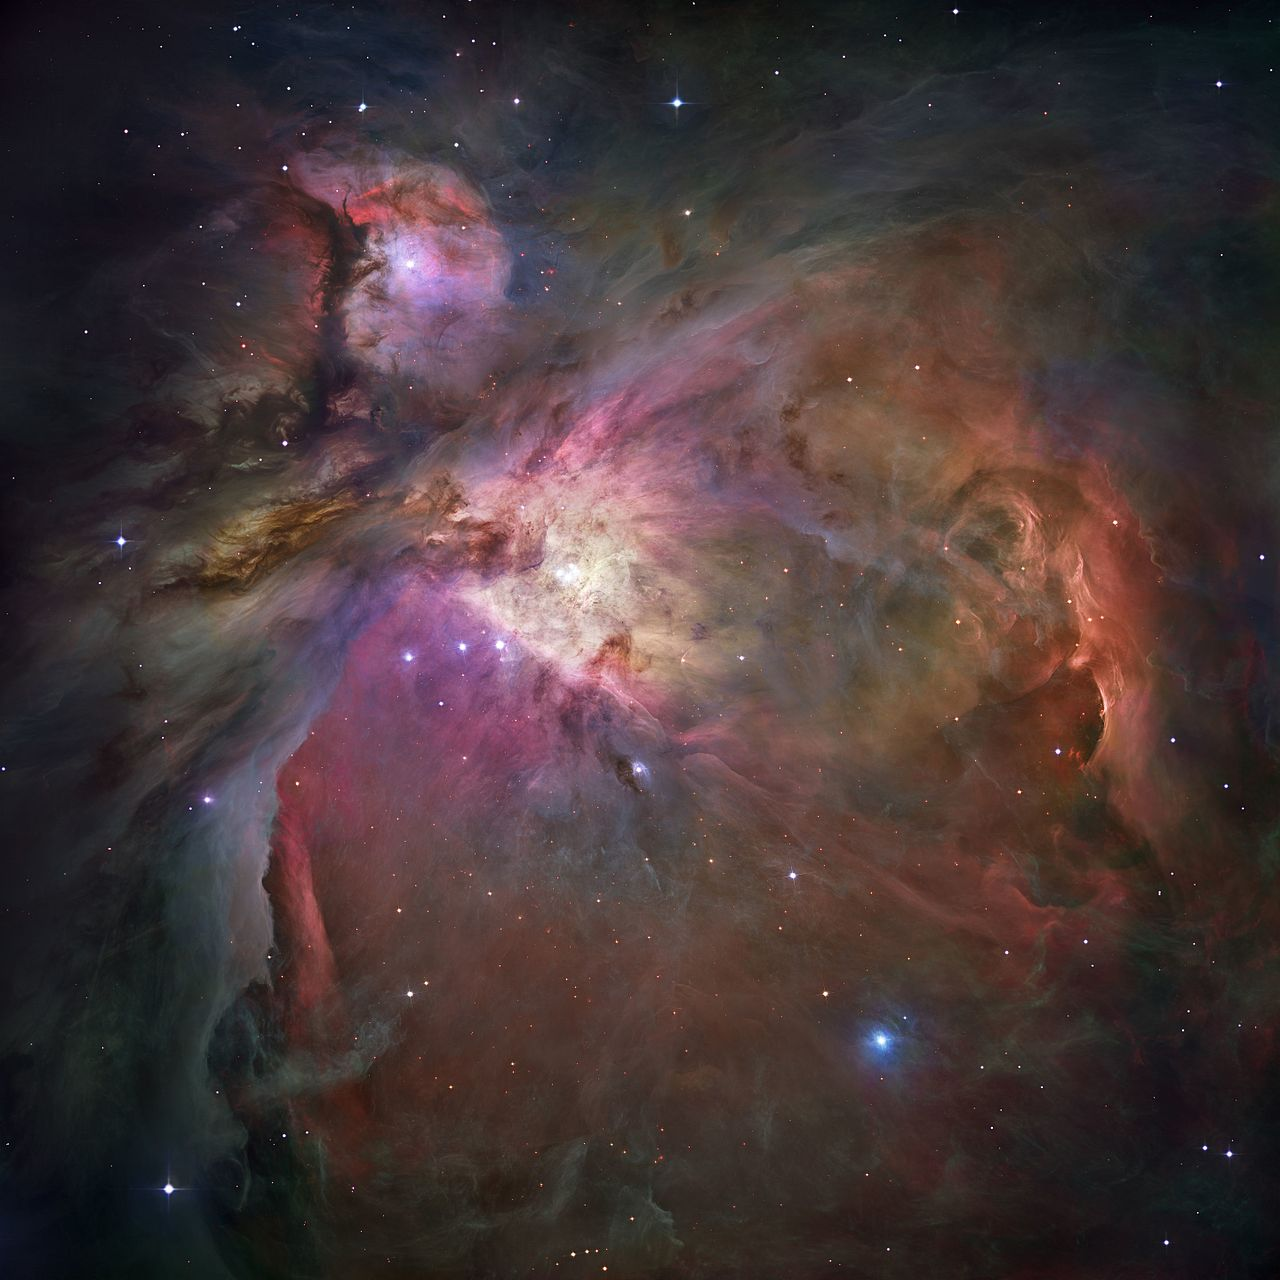
\includegraphics[]{ONCpic.png}
	\caption{The Orion Nebula in the Milky Way.}
  \end{figure}

\newpage

Do all stars have the same mass as the sun? Or is there a distribution of masses of stars in a stellar cluster i.e. a collection of stars? If yes, what does this distribution look like? Do most stars take the mass of the sun or is their some other characteristic mass where the stellar mass distribution peaks?    
 
\section{Mass Function}
Even though all stars in a stellar cluster are formed in the same environment, the process of forming a star is a stochastic/probabilistic in nature and in fact very difficult to understand. The reason being it's not just self-gravity that causes the gas to collapse and form the star but a combination of many other processes such as magnetic field, and turbulence that determine this formation. So stars formed in a molecular cloud, which is the birth place of stars, will not just have one particular mass but a spectrum of masses. And when you distribute these stellar masses in a star forming event into different mass intervals, the distribution is called the mass function. 
\\ Since stars also like us have a limited amount of of fuel in them i.e. have a finite lifetime, they die too. Or more appropriately to say  'evolve'.  The distribution of the stellar masses changes each time a star evolves. Hence, at each epoch i.e. a snippet of considerable time, your distribution of stellar masses varies. So if you got lucky one day, and say hypothetically you really happen to catch the star formation event from the beginning, the distribution you obtain at the time of birth is called the initial mass function. 


\section{Mathematical representation of  Mass function}
As we have established that stellar masses range over a continuous spectrum of masses, mathematically we can model this phenomena using a probability distribution function. 
So if $m$ is the mass of a star considered to be a continuous random variable, we can use a pdf $f(m)$, where $f(m)dm$ gives the number of stars in some volume of space in the interval $[m,m + dm]$,
\\

\begin{equation}
f(m) = \dfrac{d(N/V)}{dm}\,,
\end{equation}
where $N$ = Number of stars in the interval $[m,m+dm]$ , $V$ = Volume.
\\
But wait, there is an extremely important assumption that underlies such a modeling process. We assume that this pdf of stellar masses only depends on the mass as an input and is independent of space and time. Hence each time i.e. at each epoch you observe the stellar cluster you will get a different distribution. Also which part of the cluster you'll look at will change the distribution. So it is ideal to observe an entire stellar cluster to study the mass function. 
\\
It is a usual practice to divide the intervals for the mass function into log masses  i.e. take the pdf as $f(ln\,m)$  instead of $f(m)$ i.e. 
\begin{eqnarray}
f(ln\,m) = \dfrac{d(N/V)}{dln\,m}\, ,\\
f(ln\,m) = \dfrac{d(N/V)}{dm} \dfrac{dm}{dln\,m}\, , \\
f(ln\,m) = m\,f(m)\, , 
\end{eqnarray}

\\
$f(ln\,m)$ gives the number of stars in some volume of space in the interval $[ln\,m,ln\,m + d\,ln\,m]$.

\\
CODE example: In the following example we want to study the stellar mass distribution of the Orion Nebula Cluster (ONC)~\cite{Hillenbrand1997, DaRio2012} which is a stellar cluster in the Milky Way. The ONC.dat file contains the different stellar masses. To obtain the mass function, we plot a histogram with $f(m)$ on the y-axis which is obtained from the frequency of each mass interval.  The mass function of any stellar cluster has a characteristic peak and a power-law tail. 

\begin{lstlisting}[language=Python, caption=Python example]
''' 
    This code is developed for the Python workshop at the Winter
    School in Astronomy 2017
    
    @Author : Sayantan Auddy
    Created : 7 Feb 2017
    
    Modified : 14 Feb 2017
    
    Objective : To the study the probability denstiy 
    distribution of mass for ONC data.

'''

## for any python documentation and FAQs
## visit https://www.python.org/doc/

## Importing the numerical module numpy
## https://docs.scipy.org/doc/ 
import numpy as np  

## Importing matplotlib for plotting
## visit http://matplotlib.org/contents.html
import matplotlib.pyplot as plt 

## Scipy is scientific python 
from scipy.special import erfc

## to get the plot in a separate GUI window (not needed for 
## other platform)
# %matplotlib qt  

## this command plots the matplotlib figures in line with the 
## code this works by default in jupyter 
%matplotlib inline  

# That gives a interactive version within the notebook
# %matplotlib notebook

## read the data file in fp
## fp is a file handle
fp = open ("ONC.dat",'r')

## Declaring an empty list to store the data from the .dat file
mass =[]

## Reading the data from a .dat file line by line
## please refer to the link for details  
## http://stackoverflow.com/questions/4071396/split-by-comma
## -and-strip-whitespace-in-python

## Python reads top to bottom left to right.
for line in fp:
    #print(line.strip().split())
    #print(line.strip())
## t is a list. You can check by type(variable)
    t = line.strip().split()              
    for value in t:
        # the func append helps to modify the array storage
        # python returns a string, but we need a floating point
        mass.append(float(value))         

## closing the file after it reads in the data *important 
fp.close()  

##to convert rho python list to numpy array list for easy manipulation
mass_array = (np.asarray(mass))           


############################################################
'''
    Visualisng the nature of the data by ploting a histogram

'''

##declaring the bin size for the histogram
binsize = 50                              
plt.figure(1)

## this gives the latex text for the plots
# plt.rc('text',usetex=True)               

## Binning in d ln(mass). Binning can be modified depending 
## on the requirement of the problem
plt.hist(np.log(mass_array),binsize,normed=1,facecolor='red'
         ,cumulative=False) 

## Binning in d(mass) i.e. linear spacing
# plt.hist(mass_array,binsize,normed=1,facecolor='red'
#          ,cumulative=False) 

## x axis limit
plt.xlim(min(np.log(mass_array))-0.5,max(np.log(mass_array))+0.5) 
## y axis limit
# plt.ylim(-3,3)       
## log scale on the y axis
plt.yscale('log')                         
plt.title ("ONC mass function",fontsize=11)
plt.xlabel("ln(mass)", fontsize=12)
plt.ylabel("Frequency",fontsize=12)
plt.savefig("ONC.png",dpi = 600)
plt.show()
\end{lstlisting}



     \begin{figure}
	\centering
        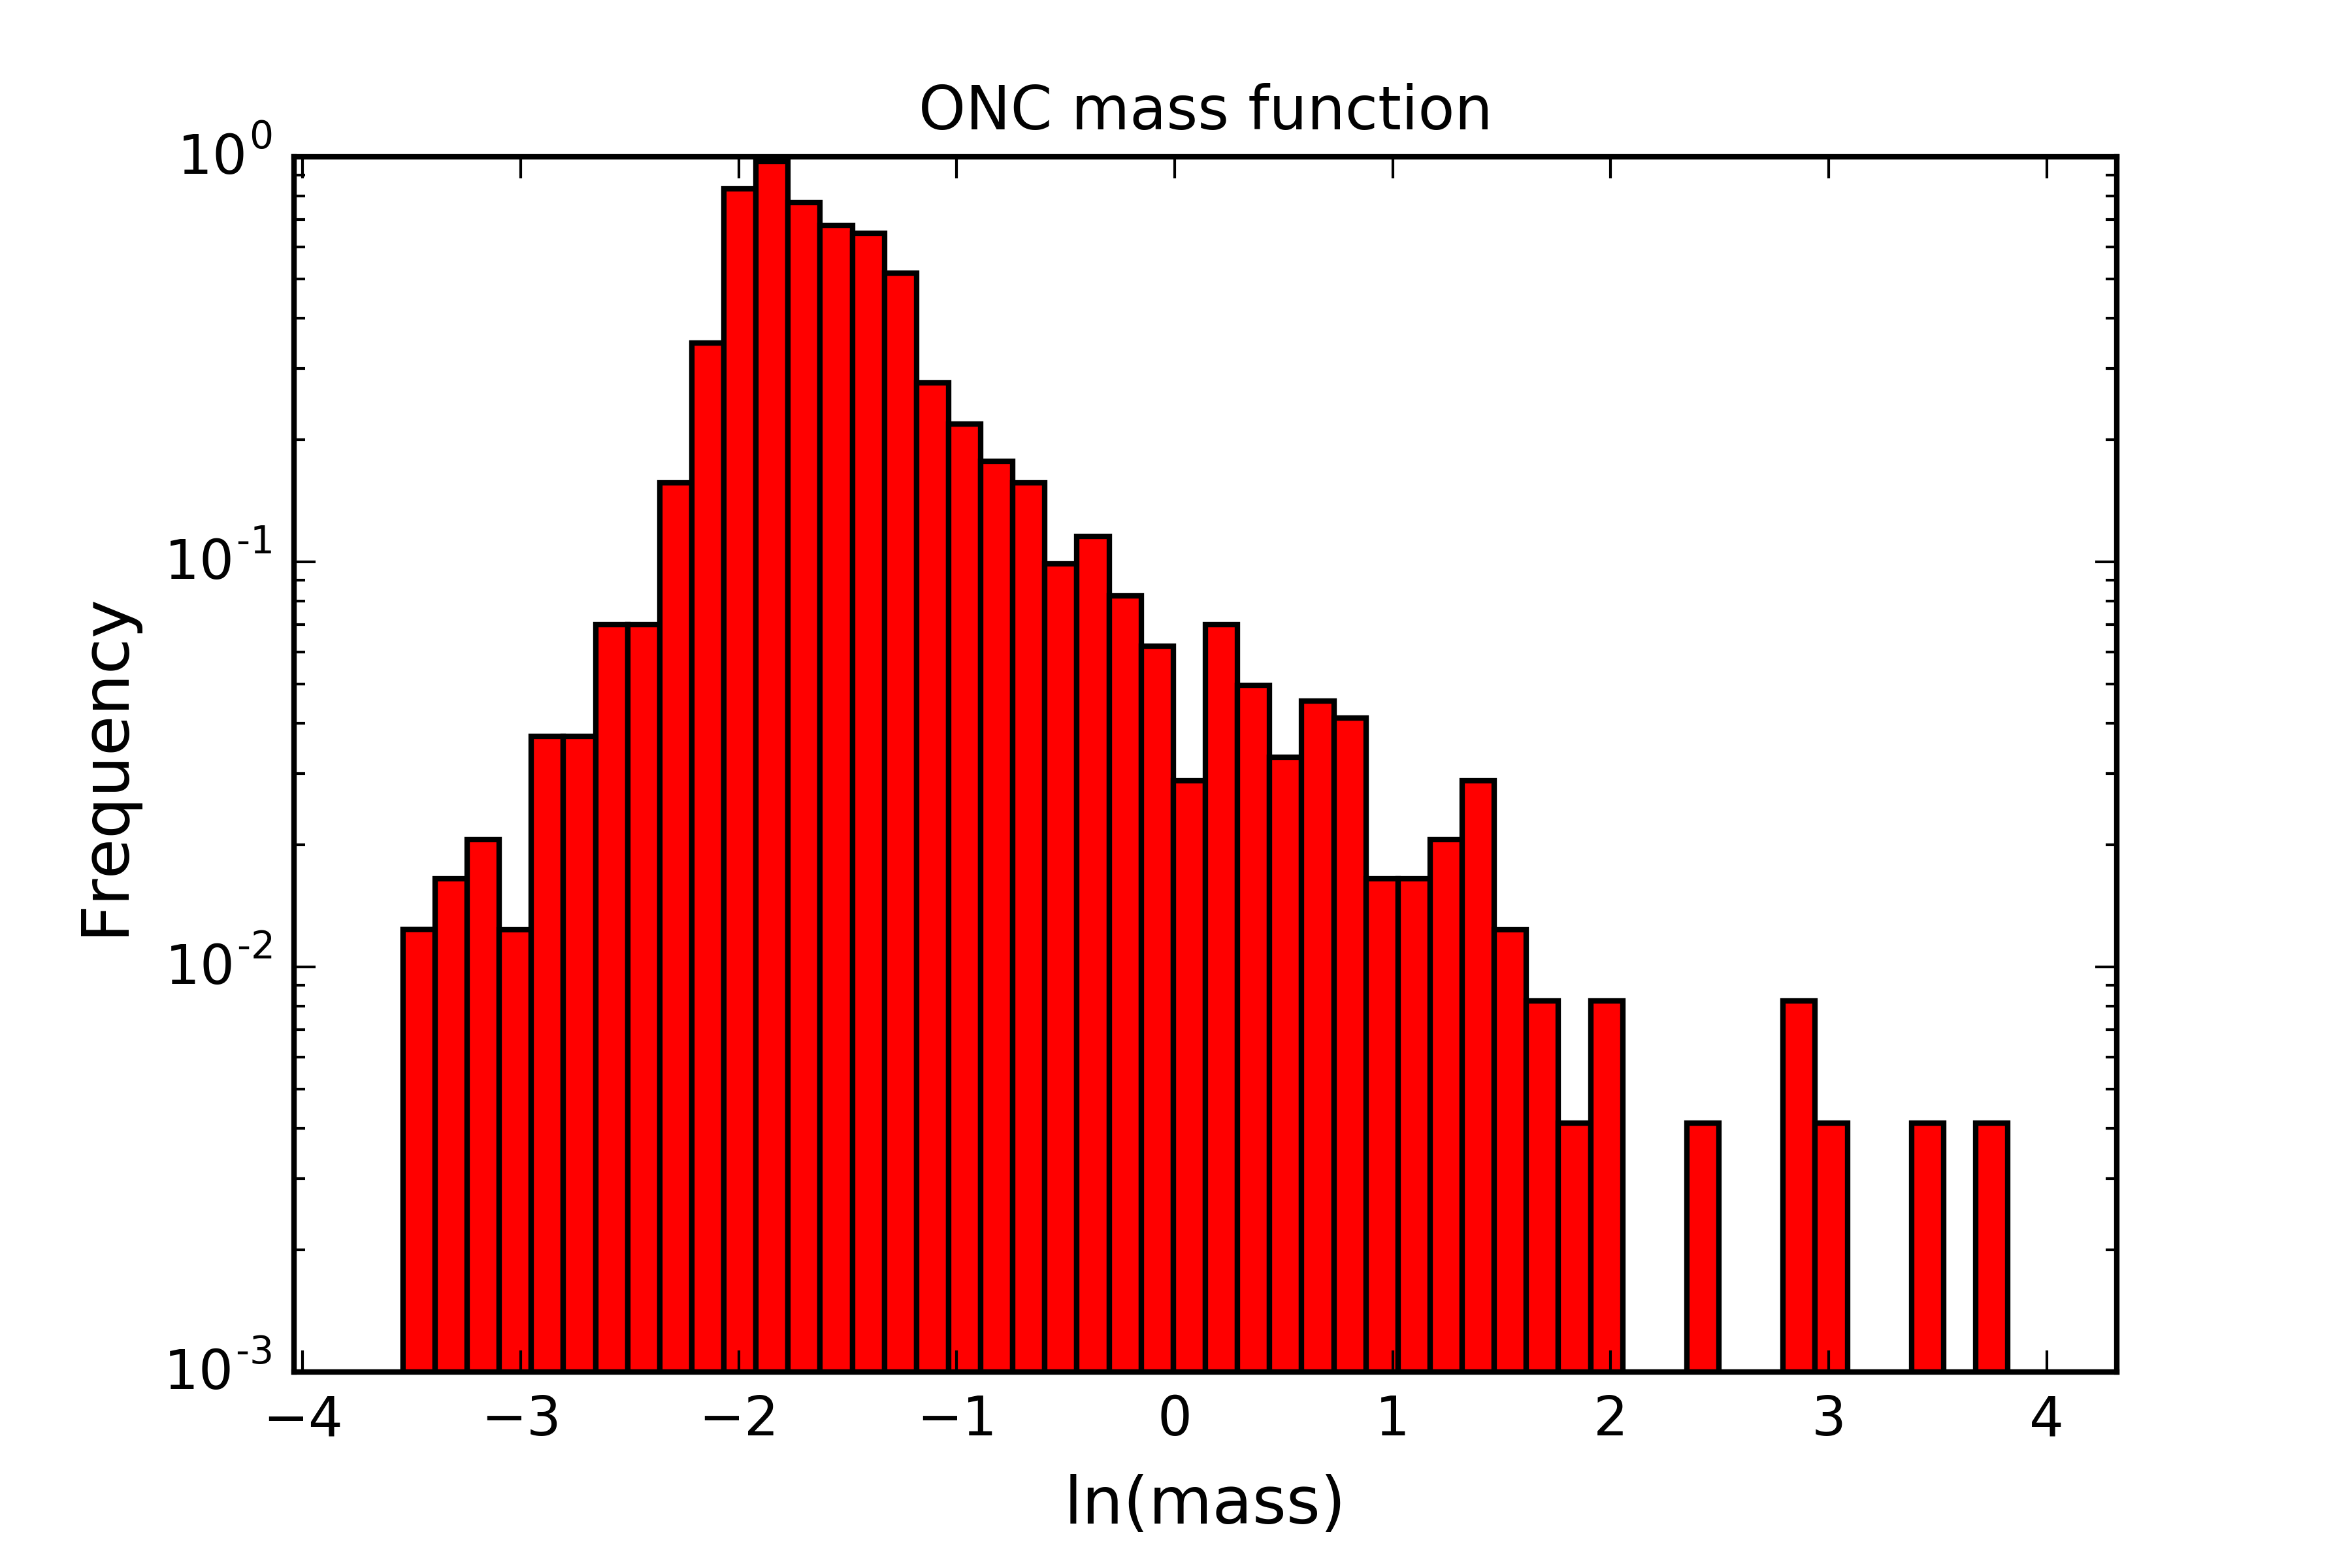
\includegraphics[]{ONC.png}
	\caption{The histogram i.e. the mass function for the stellar masses of the ONC.}
      \end{figure}

\section{Modeling the Mass function }
Since 1955, many astronomers have used various functions to model the stellar mass distribution. Salpeter (1955) was the first to provide the stellar initial mass distribution with an analytic power law pdf approximation. What he essentially did was to fit a power law or a linear function in the log-log axis since a power-law becomes a linear function in log-log. So the model he obtained was  $dN'/dm \propto m^{-\alpha}$ with $\alpha = 2.35$ or $dN'/dln\,m \propto m^{-1.35}$ over the mass range $0.4\,M_{\odot}< m<10\,M_{\odot}$. Here $M_{\odot}$ represents the mass of the sun. 

NOTE: The exponent that you obtain for $f(m)$ i.e. $dN'/dm$ is $-\alpha$ while the exponent for $mf(m)$ i.e. $dN'/dln\,m$ is $-\alpha + 1$.
The other two most commonly used models are the Chabrier functional form and the Kroupa functional form.
Chabrier modeled  the substellar and low mass stellar regime  i.e. $m < 1\,M_{\odot}$ using a lognormal function and used the Salpeter's power-law approximation for intermediate and high mass stellar regime i.e. $m > 1\,M_{\odot}$
Kroupa, on the other hand, gave a multisegment power law profile i.e. piecewise function of three power-laws for substellar, low, and high stellar mass regimes.

\section{Modified Lognormal Power-Law Probability Distribution Function}

In 2004, Basu \& Jones~\cite{Basu2004} introduced a hybrid three-parameter probability density function, the Modified Lognormal Power-Law (MLP) probability distribution function. Except for the power law approximation introduced by Salpeter that is used to model  stars above $1\,M_{\odot}$, other models like the Chabrier and Kroupa functional form need some sort of a joining condition as they are piecewise functions. The MLP on the other hand doesn't require a joining condition. Also most other commonly used functional forms lack physical justification while the MLP has an underlying physical motivation. 
Please refer to  Basu \& Jones to understand the physical motivation underlying the model.  


\subsection{PDF and Properties}
%%%% can you explain why the choice of a pdf for the distribution matters?
The MLP function is a three-parameter pdf. The three parameters of the distribution function are $\alpha_0$, $\mu_{0}$, and $\sigma_{0}$. $\alpha_0 + 1$ is the power-law index of $\dfrac{dN}{dm}$ for the power-law distribution: characteristic of a Pareto distribution which is used to represent pure power-law distributions. The parameters $\mu_{0}$ and $\sigma^{2}_{0}$ are the same as for the lognormal distribution but do not represent the mean and variance of the distribution unlike for the lognormal distribution. Parameters $\mu_{0}$ and $\sigma_{0}$ describe the shape of the lognormal-like body and $\alpha_0$ represents the power-law tail. In the limit as $\sigma_{0}$ tends to zero, the function behaves as a pure power-law. 

If $m$ is the the mass of a star, the pdf of the MLP function is given in the closed form as ~\cite{Basu2015}: 
\begin{equation} f(m) = &\frac{\alpha_0}{2}\exp\left(\alpha_0\mu_0 +\alpha_0 ^2\sigma_0 ^2 / 2\right)m^{-(1+\alpha_0)} \notag \times \erfc\left(\frac{1}{\sqrt{2}}\left(\alpha_0\sigma_0 - \frac{\ln m - \mu _0}{\sigma_0}\right)\right) \ , \ m \in[0,\infty) \ , \label{MLP} \end{equation}

\\Some properties of the MLP function are: \\
(i) Raw Moments:\begin{equation} E[M^k] =\frac{\alpha_0}{\alpha_0 - k} \exp\left(\frac{\sigma_0^2k^2}{2} + \mu_0 k\right) \label{MLPMomemnts} , \ \alpha_0 > k. \end{equation}
(ii) Variance: 
\begin{equation} \label{var} \notag \text{Var}(M) &= E[M^2] - (E[M])^2 \\ &= \alpha_0 \exp(\sigma_0^2 + 2\mu_0)\left(\frac{e^{\sigma_0^2}}{\alpha_0-2} -  \frac{\alpha_0}{(\alpha_0 - 1)^2}\right), \ \alpha_0 > 2.
\end{equation} 
(iii) Cumulative Distribution Function:
\begin{equation} F_M(m;\alpha_0,\mu_0,\sigma_0) &= \frac{1}{2}\erfc\left(-\frac{\ln(m)-\mu_0}{\sqrt{2}\sigma_0}\right) -\frac{1}{2}\exp\left(\alpha_0\mu_0+\frac{\alpha_0^2\sigma_0^2}{2}\right)m^{-\alpha_0}\erfc\left(\frac{\alpha_0\sigma_0}{\sqrt{2}}-\frac{\ln(m)-\mu_0}{\sqrt{2}\sigma_0}\right). %\label{cumDist} 
\end{equation}
(iv) Mode: Solving the following transcendental equation will give us the mode of the distribution
%
\begin{equation} f'(m) = 0 \iff K\erfc(u) = e^{-u^2} \label{modeEq}  \ , \end{equation}
%
where 
\begin{equation} K &= \sigma_0(\alpha_0 + 1)\sqrt{\frac{\pi}{2}}\,, 
&u=\frac{1}{\sqrt{2}}\left(\alpha_0\sigma_0 - \frac{\ln m - \mu _0}{\sigma_0}\right).
\end{equation}
%



\section{Model Fitting}
 Model fitting investigates whether a mathematical model can be used to describe a given data set. Here we check whether the MLP can be used to describe the underlying stellar mass distribution. To do so we use non-linear regression/curve fitting. Regression essentially finds best fit values for the unknown model parameters by minimizing the  sum of the squared errors.  
 From the mass function of the ONC which is the normalized histogram obtained above, we can consider the centre of each bin in the histogram and the bin height corresponding to the value for $f(m)$ as our corresponding data points.

CODE: The following code demonstrates obtaining the data points for $m, f(m)$ or $m, mf(m)$ from the histogram depending whether binning in linear or log scale. 

\begin{lstlisting}[language=Python, caption=Python example]
## To fit the histogram using the least square method
## this gives the frequency and the edges of the bins

## important to note we bin in d mass (linearly spaced)
# bincount,bin_edge = np.histogram(mass,binsize,normed=1) 

## important to note we bin in d ln(m) (logarithmically spaced)
bincount,bin_edge = np.histogram(np.log(mass_array),binsize,normed=1) 

## bincenter is the value for the center of each bins
bincenter = (bin_edge[1:]+bin_edge[:-1])/2.0
xdata=bincenter[:]
ydata=bincount[:]
plt.figure(2)
# plt.ylim(10**-1,10**3)
plt.ylabel('ln (mf(m))')
plt.xlabel('ln(m)')
plt.plot(xdata,ydata,'ro',markersize=3)
plt.yscale('log')
plt.savefig("ONCMassfunc.png",dpi = 600)
\end{lstlisting}


     \begin{figure}
	\centering
        \includegraphics[]{ONCmassfunc.png}
	\caption{The data points obtained from the histogram of the ONC.}
      \end{figure}

CODE: We then define the MLP function. Note in the following definition we use $mf(m)$ instead of $f(m)$ and hence the exponent in the above definition of the MLP is $-\alpha_0$ instead of $-(1+\alpha_0)$. Regression is used to obtain the best fit parameters for the underlying stellar mass distribution of the ONC. 

\begin{lstlisting}[language=Python, caption=Python example]
''' 
    We will use least square method to fit MLP to the mass data of 
    the ONC cloud. Curve Fit is the funtion in python
    which uses non-linear least squares to fit a function, f, to data.
    A statistical method used to determine a line of best fit
    by minimizing the sum of squares created by a mathematical function.
    A "square" is determined by squaring the distance between a data point 
    and the regression line.

'''

def MLPcurvefit(x,alpha,mu0,sigma0):
    """
        General overview of the function
        This is MLP function f (m) which is used to fit the data using 
                least square method 
        Inputs: An array of x values and the parameter 
                alpha, mu_{0} and sigma_{0}
        Output: Best fit parameters
        Reference : Basu et al 2015. 
        Author: Sayantan
    """
    p1=(alpha/2.0)*np.exp(alpha*mu0+((alpha*sigma0)**2)/2.0)
    p2=x**(-(1+alpha))
    arg=(1.0/np.sqrt(2.0))*(alpha*sigma0-(np.log(x)-mu0)/sigma0)
    p3=erfc(arg)
    p = p1*p2*p3;
    return(p)

## imoporting the curve_fit function from scipy module
from scipy.optimize import curve_fit


##important to note we bin in d(m)
bincount_ls,bin_edge_ls = np.histogram(mass_array,binsize,normed=1) 

# bincenter is the value for the center of each bins
bincenter_ls = (bin_edge_ls[1:]+bin_edge_ls[:-1])/2.0
fitParams,fitCov=curve_fit(MLPcurvefit,bincenter_ls,
                           bincount_ls,bounds=([0.,-3,0,],[5., 5., 5.]))
print('alpha=%f\n'%(fitParams[0]))
print('mu_0=%f\n'% (fitParams[1]))
print('sigma_0=%f\n'%(fitParams[2]))
\end{lstlisting}

RESULT: 

alpha=1.552174

mu_0=-2.306813

sigma_0=0.770617


\subsection{Maximum Likelihood Estimation}

A more robust method of fitting a model to data points is by using maximum likelihood estimation. Given a sample of data points $x_1,\,x_2,\,x_3,\,.....,\,x_n$ assumed to be taken from a pdf $f(X\,|\Theta)$ of $k$ unknown parameters $\theta_1,\,\theta_2,\,.......,\,\theta_k$, we can define the likelihood function. 
\begin{equation}
L(\Theta\,|x_i) =  f(x_1\,|\Theta)\into f(x_2\,|\Theta) \into .....\into f(x_n\,|\Theta) = \prod_{i=1}^{n} f(x_i\,|\Theta)\,,\\
\end{equation}
Note that $L(\Theta\,|x_i)$ is a function of the unknown parameters with data points kept fixed unlike the pdf which is a function of observations with fixed parameter values. 
Maximizing the likelihood function helps in finding the parameter values that are most likely to describe the data set. \\
For simplicity the log of the likelihood function is maximized i.e.: 
\begin{equation}
\ln\,L(\Theta\,|x_i) =  \ln\,f(x_1\,|\Theta) +\,\ln\,f(x_2\,|\Theta) +\, .....+\,\ln\, f(x_n\,|\Theta) = \sum_{i=1}^{n} \ln\,f(x_i\,|\Theta)\,,\\
\end{equation}

One can find maximum likelihood estimator for the parameters $\theta_1,\,\theta_2,\,.......,\,\theta_k$ by simultaneously solving for: 
\begin{equation}
\dfrac{d\,\ln\,L(\Theta\,|x_i)}{d\theta_j}\,=\,0 \, : j = 1,....,k\,.
\end{equation}
For various distributions like the lognormal distribution or the Pareto distribution, functional forms can be found for the maximum likelihood estimators but for distributions that do not have an analytic form for the estimators, global optimization techniques such as basin hoping or differential evolution are explored to find global minima for the negative-likelihood function i.e. $ - \ln\,L(\Theta\,|x_i) $ which is same as finding global maxima for the likelihood function. \\
CODE: We first need to define the likelihood function for the MLP function corresponding to the definition given above in equation 9 and 10.
\begin{lstlisting}[language=Python, caption=Python example]

## Declaring MLP maximum likelihood function. Please refer to the
## following reference for details.


def MLPMLEfit(params):
    """
        General overview of the function
        This is the maximum likelihhod of the MLP function. 
        Inputs: The data point are loaded as inputs
        Output: On optimising this function it gives the best fit paramters
                alpha, mu_{0} and sigma_{0}
        Reference : Please read section () for details
        Author: Sayantan
    """
    alpha,mu0,sigma0=params
    x = mass_array              # the data is loaded
    p1=(alpha/2.0)*np.exp(alpha*mu0+((alpha*sigma0)**2)/2.0)
    p2=x**(-(1+alpha))
    arg=(1.0/np.sqrt(2.0))*(alpha*sigma0-(np.log(x)-mu0)/sigma0)
    p3=erfc(arg)
    p = p1*p2*p3;
    return sum(-np.log(p))     # retuns the log likelihood. 
\end{lstlisting}

CODE: We then optimize the log likelihood function using 2 methods i.e. differential evolution and basin hopping. The following is code for differential evolution.

\begin{lstlisting}[language=Python, caption=Python example]
'''
    For optimization we shall use
    scipy.optimize.differential_evolution

    Finds the global minimum of a multivariate function. 
    Differential Evolution is stochastic in nature (does not use gradient
    methods) to find the minimium, and can search large areas of candidate
    space, but often requires larger numbers of function evaluations than 
    conventional gradient based techniques.
    For detials: 
    https://docs.scipy.org/doc/scipy-0.18.1/reference/generated/
    scipy.optimize.differential_evolution.html

'''
## We want to find the optimized value for the parameters alpha,
## mu0 and sigma0 for the best
## fit MLP fucntion.

## importing the differential_evolution routine from scipy module
from scipy.optimize import differential_evolution
## defining the possible bounds for the values of alpha, mu0 and sigma0
bounds = [(1, 5), (-3, 1),(0.01,2)]

np.random.seed(1)   # fixed seed gives the same values on every run

result = differential_evolution(MLPMLEfit, bounds)
## result.x, result.fun
print("global minimum: x = [%.3f, %.3f,%.3f], f(x0) = %.3f\n" % 
      (result.x[0], result.x[1],result.x[2],result.fun))
print('alpha  = %.3f\n'%(result.x[0]))
print('mu0    =%.3f\n'%(result.x[1]))
print('sigma_0= %.3f\n'%(result.x[2]))
\end{lstlisting}

RESULT: global minimum: x = [1.403, -2.084,0.348], f(x0) = -789.658

alpha  = 1.403

mu0    =-2.084

sigma_0= 0.348

CODE: Optimization using Basin Hopping is demonstrated below. 

\begin{lstlisting}[language=Python, caption=Python example]

'''
For optimization we shall use
scipy.optimize import basinhopping
For detials: 
https://docs.scipy.org/doc/scipy-0.18.1/reference/generated/scipy.
optimize.basinhopping.html

'''
from scipy.optimize import basinhopping

## intial guess values of the parameter alpha, mu0, sigma0
x0 = [3., 0.1,0.1]

## defining the possible bounds for the values of alpha, mu0 and sigma0

xmin = [1.,-3.,0.]          # lower bound
xmax = [5.,1., 1.]          # upper bound

## rewrite the bounds in the way required by L-BFGS-B
bounds = [(low, high) for low, high in zip(xmin, xmax)]

BHsettings = dict(method="L-BFGS-B", bounds=bounds)

ret = basinhopping(MLPMLEfit,x0,minimizer_kwargs=BHsettings,
                   niter=200,disp=0,niter_success=None)

print("global minimum: x = [%.3f, %.3f,%.3f], f(x0) = %.3f\n" % 
      (ret.x[0], ret.x[1],ret.x[2],ret.fun))
print('alpha  = %.3f\n'%(ret.x[0]))
print('mu0    =%.3f\n'%(ret.x[1]))
print('sigma_0= %.3f\n'%(ret.x[2]))
\end{lstlisting}

RESULT: global minimum: x = [1.421, -2.071,0.351], f(x0) = -790.021

alpha  = 1.421

mu0    =-2.071

sigma_0= 0.351

CODE: Once the best fit values of the unknown parameters are found using regression and maximum likelihood we finally visualize the mass function with the MLP fits. 

\begin{lstlisting}[language=Python, caption=Python example]
'''
    Plotting the MLP with the best fit parameters along with
    the ONC data points.

''' 
# using the best fit parameters from the curve fit least square method
params_ls = fitParams[0],fitParams[1],fitParams[2]
# using the best fit parmameters from differential evolution optimisation
params_dff = [ret.x[0],ret.x[1],ret.x[2]]
# using the best fit parameters from the basinhopping optimisation
params_bh = result.x[0],result.x[1],result.x[2]

# defining an array of numbers to plot the MLP function
xarray = np.logspace(-1.5,1.6,1000)
# plt.hist(np.log(mass_array),binsize,normed=1,facecolor='blue'
#          ,cumulative=False) 
plt.figure(3)
plt.clf()
plt.plot(xdata,ydata,'ro',markersize=3,label="ONC data")
plt.plot(np.log(xarray),MLP(xarray,*params_ls),'g-',label='LS')
plt.plot(np.log(xarray),MLP(xarray,*params_dff),'k',label='DE')
plt.plot(np.log(xarray),MLP(xarray,*params_bh),'b--',label='BH')        
plt.legend(numpoints=1,fancybox=True,shadow=True,fontsize=10)
plt.xticks(fontsize=12)
plt.yticks(fontsize=12)
plt.title (r'ONC mass density PDF',fontsize=14)
plt.xlabel('ln(m)',fontsize=14)
plt.ylabel('ln(m f(m)',fontsize=14)
# plt.text(-2,0.001,r'$\sin(x)$',fontsize=12)
plt.yscale('log')
plt.savefig("MLPfits",dpi = 600)
plt.show()
\end{lstlisting}

     \begin{figure}
	\centering
        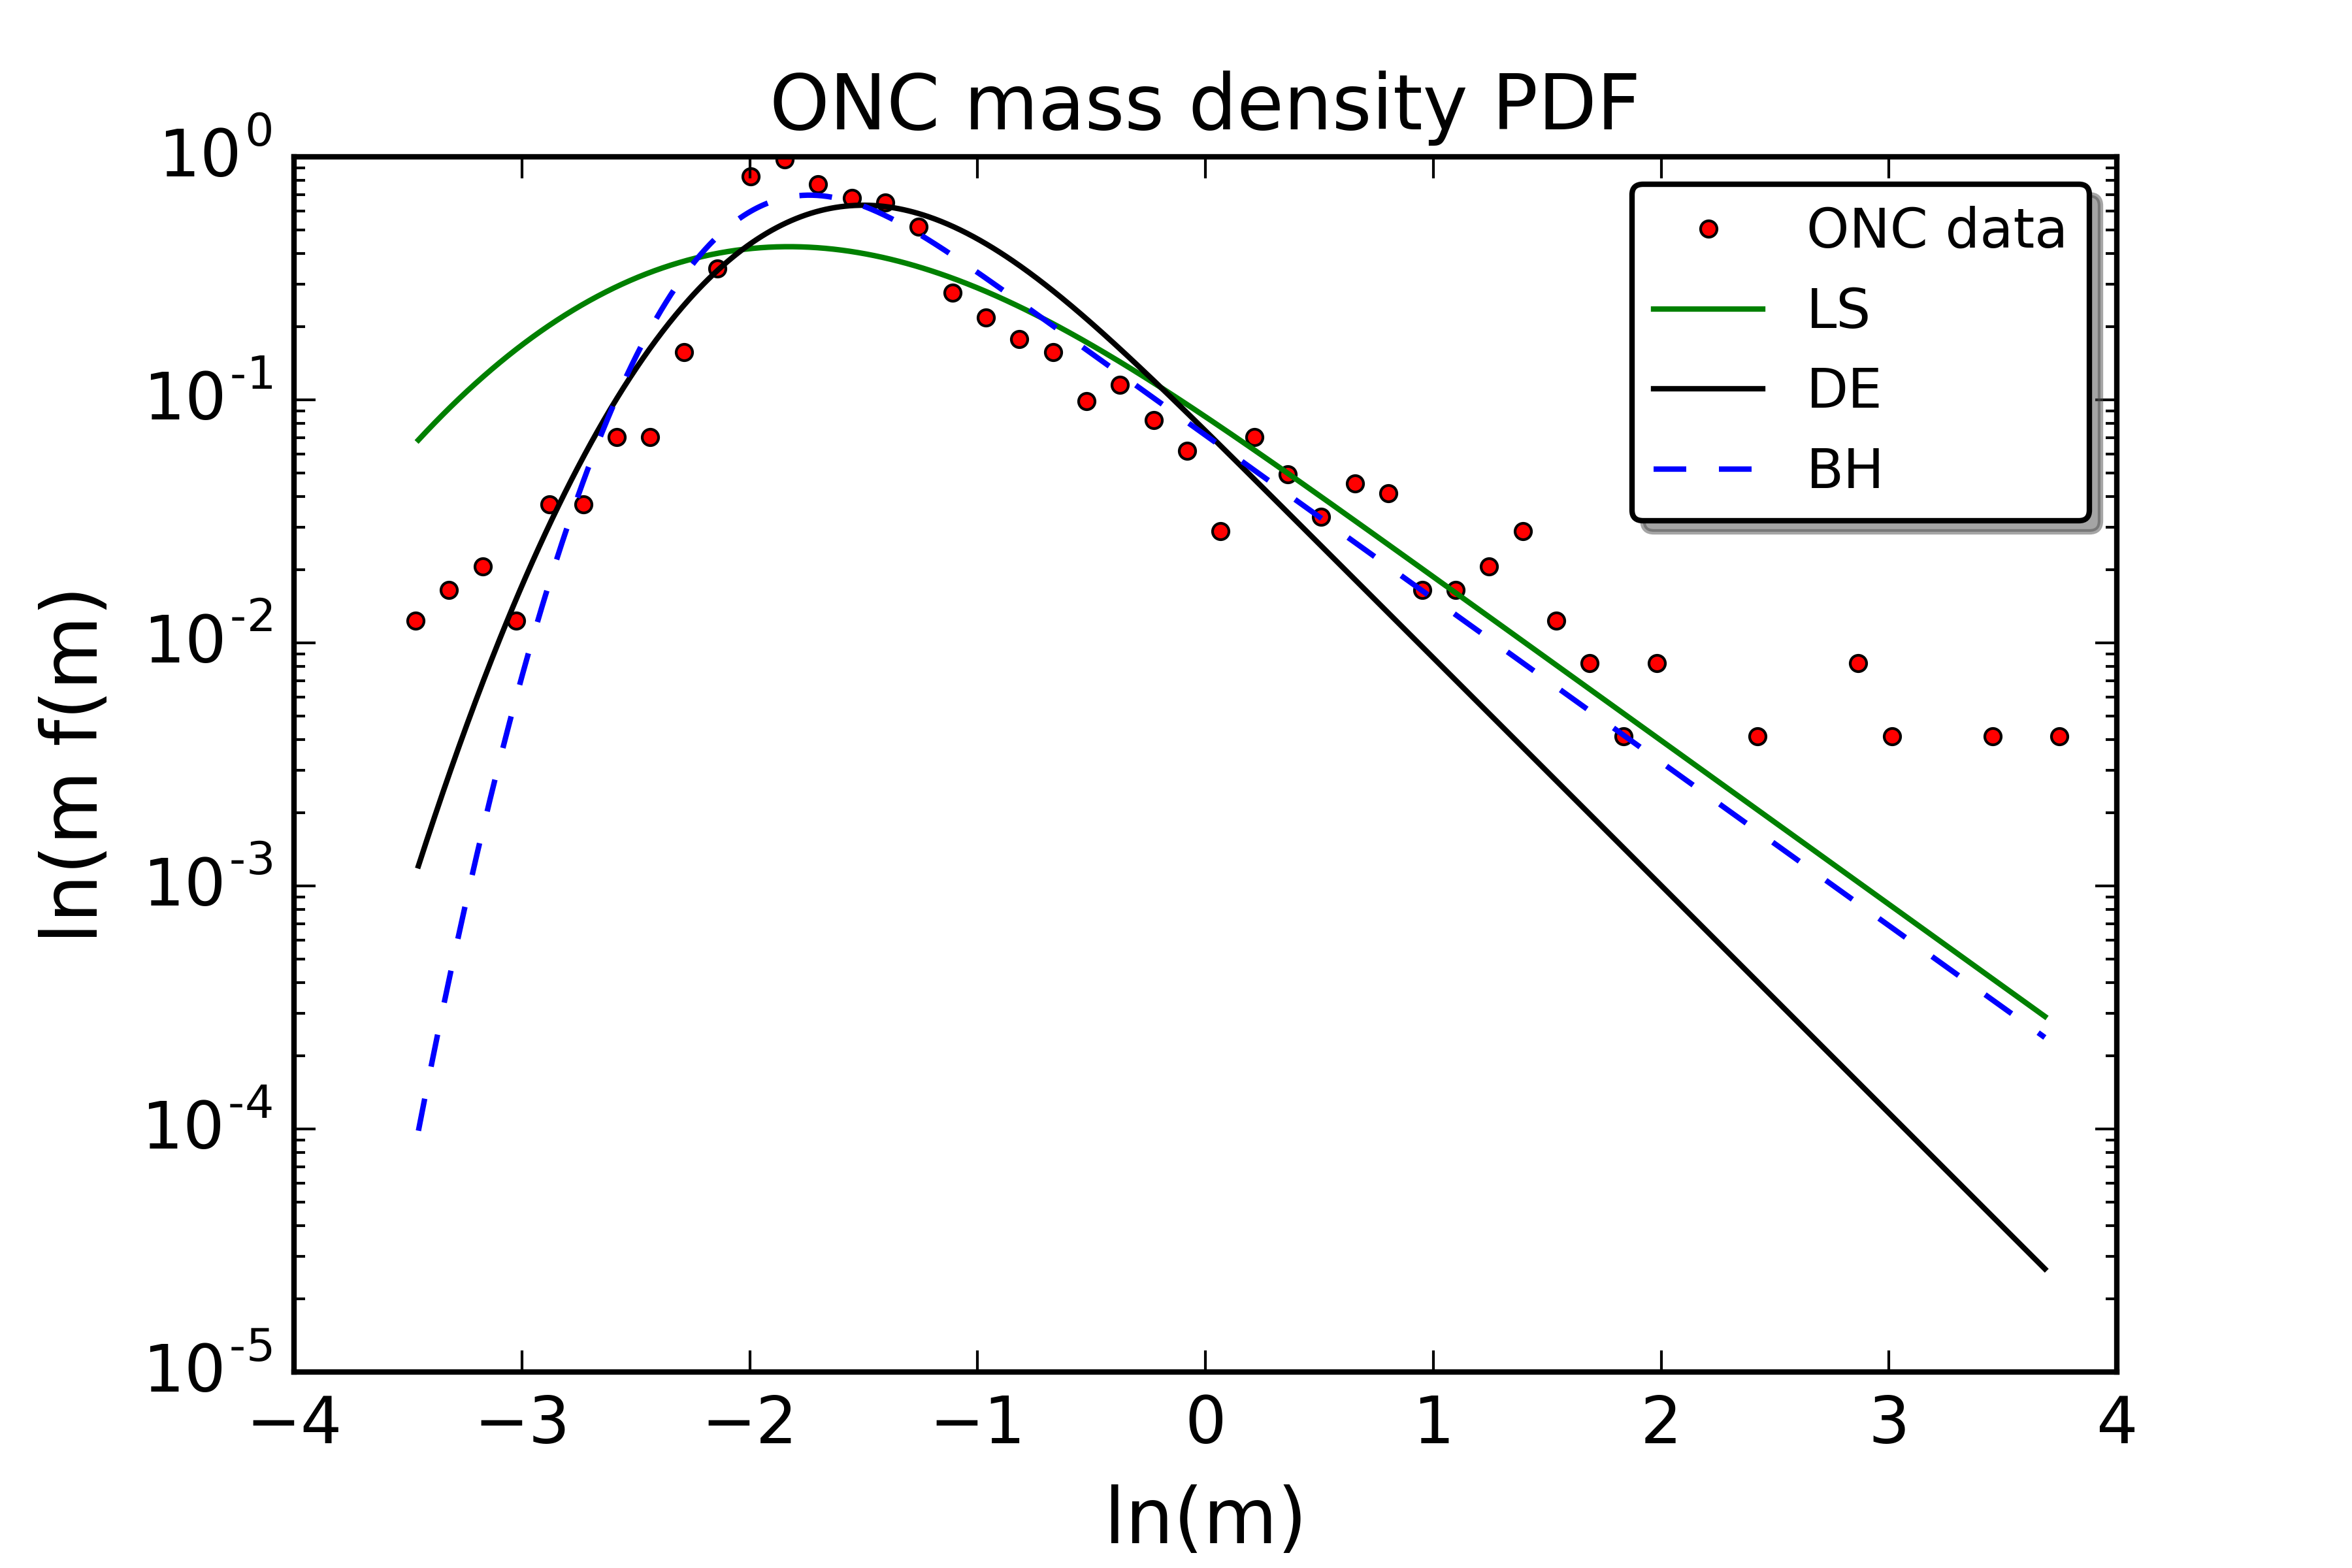
\includegraphics[]{MLPfits.png}
	\caption{Plotting the mass function of the ONC with the MLP fits.}
      \end{figure}


\bibliographystyle{unsrt}
\bibliography{ref}{}

 \\Image Source: http://hubblesite.org/news\_release/news/2006-01

%\lstinputlisting[language=Python]{Wintersch_workshop.py}
\end{document}